\cleardoublepage
\chapter{Implementation}
\label{ch:implementation}
Chapter 4 describes the implementation of the thesis.
This includes how the thesis group chose to implement the design discussed in previous chapters, and the research methods used to arrive at design decisions.

\section{REST API}\label{sec:REST API}

The API exposes several endpoints that allows for saving an image and a receipt to a database.
The API is also connected to the ML and OCR module.

\section{Web solution}\label{sec:Web solution}

The web solution is made with React in JavaScript.
The purpose of the web solution is to give the user an interface where they can upload an image of a receipt.
And get the corresponding data from the image, and then send in the receipt with the data from the image.
This is to make the process of entering the data less time consuming.

When the user uploads an image, the web solution sends a POST request to the API, then the API saves the image to
the database.
When the image is saved, the image is sent to the OCR for text recognition.
If the output makes sense the data is returned and displayed to the user.
Then if the returned data is correct the user can then upload the receipt to the database.

\section{Dataset}\label{dataset}

The dataset provided by Simployer consists of 1194 unlabeled images and pdfs.
However, the variance of the types of receipts in the dataset is very large.
Because of this, we end up with a very small amount of images of each type after labeling them.
The dataset also includes receipts in several languages, mainly norwegian, english and polish.
We filtered the dataset to only include norwegian receipts and removing images of bad quality.
At the end of this process, the amount of usable data was very small.
The original dataset of 1194 images has been filtered down to 91 images, split into three different types of receipts.

\section{Pre-processing}\label{pre-processing}

\subsection{Data augmentation}\label{data augmentation}
Because of the low amount of images in the filtered dataset, data augmentation has to be done in order to give us enough images to be able to effectively train the CNN.
We used an open source data augmentation tool for images for this task LINK.
The augmentor takes a directory of images and applies a series of transformations on the images like scaling, skewing and rotating.
This creates copies of the images with slight differences, increasing the size of our dataset.
After applying enough transformations, the size of the dataset grew from 91 images to 1500.

\subsection{Image preparation}\label{imgprep}
Many of the images in the dataset are taken in different resolutions.
In order to prepare the images to be passed forward to the CNN model, the images resolution is rescaled to 60x60 pixels.
This significantly reduces the training time required by the network with minimal to no loss in accuracy.
The images are also converted to grayscale instead of RGB.
This reduces the amount input nodes required by the network, as each pixel will have one value instead of three.

\section{Convolutional Neural Network}\label{sec:cnn}

Our CNN is implemented using Keras.
Keras is a library for tensorflow that allows for the creation of neural network models with only a few lines of code.
The model consist of an input layer, two hidden layers, and an output layer.
The input layer and first hidden layer are 2D convolutional layers with 32 and 64 filters.
The second hidden layer and the output layer are dense layers, where the hidden layer has 64 filters and the output layer has 3 filters.
The activation function of the first three layers is Rectified Linear Unit (ReLU), while the output layer uses the sigmoid function.
Maxpooling2D is used to define a stride of 2.
This means that we take the biggest number with something thats called a max operation.
We combine the results to get a 2x2 max pool output, down from a 4x4 format.
As illustrated below.

\begin{figure}[h]
    \center{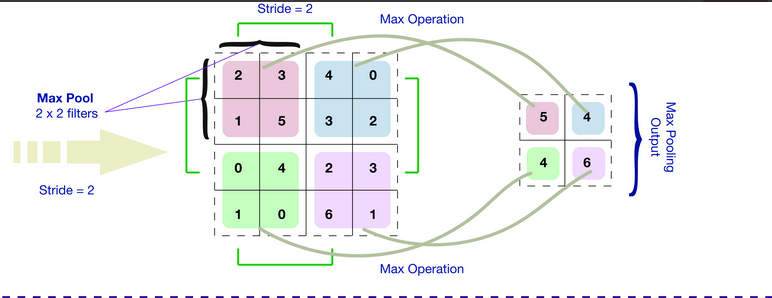
\includegraphics[width=0.65 \textwidth]{Images/maxpooling2D}}
    \caption{Overview for max pooling (Image from https://www.quora.com/What-is-max-pooling-in-convolutional-neural-networks)}
    \label{fig:figure6}

\end{figure}

We have also used batchnormalixation with the default settings in the input and hidden layers of out model.
This means that the model is sharding the data in batches.
This in turn lets us train the model with a lot less trainingsteps, and it gives us even better accuracy.
The last function we will talk about in the input and hidden layers are the dropout function.
This function will force the model to drop random filters during the training.
This will force an adaption in the model that makes it more versatile.
This is because the model can't just rely on one good path to carry its accuracy.
Therefore, it will end up with a more generic understanding of the data and avoid an overfitting.

\begin{figure}[h]
    \center{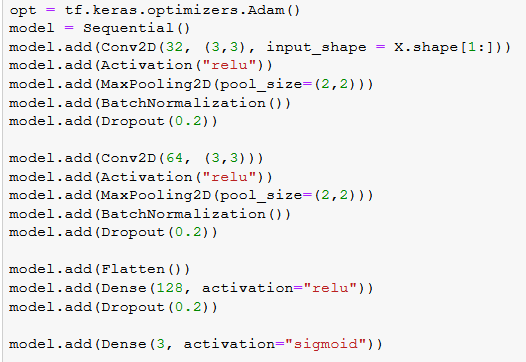
\includegraphics[width=0.65 \textwidth]{Images/CNN_model}}
    \caption{CNN model}
    \label{fig:figure4}

\end{figure}

In the compile function we defined we choose to use cross-entropy as our loss function.
Because this is the best for multiclass classification.
The optimizer is the standard adam optimizer.



\begin{figure}[h]
    \center{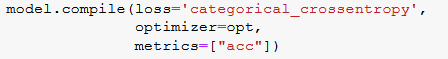
\includegraphics[width=0.65 \textwidth]{Images/CNN_compile}}
    \caption{CNN model compile}
    \label{fig:figure5}

\end{figure}






